\chapter{Komponenten}
\label{chap:komponenten}

Ein Expertensystem besteht, wie im~\hyperref[sec:anhang:tutorial_dokument]{Tutorial} unter Kapitel 2 beschrieben, aus mehreren Komponenten. Es sind dies eine Wissensdatenbank, welche die Fakten des Problembereiches in formaler Sprache enthält, ein Verarbeitungsmechanismus zum automatischen Ziehen von Schlüssen (Inferenz-Maschine) sowie eine Benutzerschnittstelle. Wie in~\autoref{ssubsec:vorgehen:grundlagen:technisch} erwähnt, ist die Verwendung eines Werkzeuges zur Modellierung einer Ontologie sinnvoll.

Das nachfolgende Kapitel gibt einen Überblick über die während dieser Arbeit verwendeten Komponenten und Werkzeuge.

Wie in der Aufgabenstellung erwähnt, sollte die Wissensmodellierung ursprünglich mit Hilfe von Apache Stanbol umgesetzt werden. Während der Arbeit wurde erkannt, dass diese Technologie für die vorgesehene Aufgabe nur bedingt sinnvoll ist. In Apache Stanbol ist es möglich die modellierte Wissensdomäne zu importieren. Das Modell wird als Ontologie in Form von Tripeln gespeichert. Die Objekte, deren Eigenschaften sowie Relationen lassen sich allerdings nicht verwalten.

Um Fragen an die Wissensdatenbank stellen zu können, ist eine entsprechende Schnittstelle notwendig. Diese wird von Stanbol in Form eines SPARQL-Endpoints zur Verfügung gestellt. Der SPARQL-Endpoint nutzt jedoch die ContentHub-Komponente von Stanbol als Datenbasis und diese stellt nur gewonnenes Wissen durch angereicherte Inhalte, aufgrund von Ontologien und Regeln, zur Verfügung.

Nach einiger Recherche stellt sich heraus, dass es zwar möglich ist andere Datenquellen für den SPARQL-Endpoint zu nutzen, dies würde jedoch erheblichen Mehraufwand in Form einer eigenen Implementation bedeuten.

Somit ist Stanbol für diese Arbeit nicht das geeignete Produkt. Nach einigen Recherchen wurden zwei Werkzeuge gefunden, welche als Ersatz für Stanbol genutzt werden können: \textit{Protégé} der Universität Stanford sowie \textit{Stardog} der Firma Clark \& Parsia. Mit einer Kombination der im nächsten Abschnitt beschriebenen Werkzeuge können alle Bedürfnisse abgedeckt werden.


\section{Stanford Protégé}
\label{sec:komponenten_protege}
Protégé ist eine Entwicklungsumgebung für Ontologien. Es wurde von der Universität Stanford entwickelt und findet in der Fachwelt häufig Anwendung. Protégé unterstützt sowohl die Modellierung von Ontologien, wie auch das Reasoning mittels verschiedener Reasoner.

\subsection{Merkmale}
\label{subsec:komponenten_protege_features}
In Protégé können die Ontologien in unterschiedlichen Schreibweisen, wie zum Beispiel OWL oder RDF/XML abgespeichert werden. Protégé erlaubt den Import und Export solcher Dateien. Die Entwicklungsumgebung bietet verschiedene Ansichten auf dieselbe Ontologie. \\
Neben dem Anlegen und Bearbeiten einer Ontologie können in Protégé Version 5.0.0 Beta 16 SWRL-Regeln hinzugefügt werden. Diese werden von Protégé direkt in der Ontologie abgelegt. 

Durch das SPARQL-Modul bietet Protégé die Möglichkeiten Abfragen in der Ontologie zu stellen. So können Informationen aus der Ontologie abgefragt werden. Ist zusätzlich ein Reasoner-Modul geladen und aktiviert, kann die Umgebung Inferenzen bei Abfragen einbeziehen. Es können verschiedene Reasoner, so zum Bespiel FACT ++ oder Pellet genutzt werden (siehe:~\ref{subsec:komponenten_reasoner}).

(vgl.~\cite{protegeFeatures})

\subsection{Ansichten}
\label{subsec:komponenten_protege_view}

Die Benutzerfreundlichkeit von Protégé wird unter Anderem dadurch erreicht, dass verschiedene Sichten auf eine Ontologie geboten werden. Neben der Entitätsansicht (Entity-View, diese enthält sämtliche Elemente einer Ontologie) existiert für alle Elementtypen wie Klassen, Dateneigenschaften und Individuen eine eigene Ansicht.

Alle Ansichten sind als Baumstruktur organisiert. Dies bietet eine klare Übersicht und ermöglicht eine hierarchiegetreue Abbildung des dahinterliegenden XML-Dokumentes.

Neben der Darstellung der im XML-Dokument abgespeicherten Informationen bietet Protégé noch andere Ansichten. So kann der Graph einer Ontologie OntoGraf-Ansicht angesehen werden.~\cite{protegeView}

Schlussfolgerungen des gewählten Reasoners werden in allen Ansicht direkt zur Laufzeit ergänzt.

\section{Clark \& Parsia Stardog}
\label{sec:komponenten_stardog}
Bei Stardog handelt es sich um eine Graphdatenbank mit Unterstüztung des RDF-Graphenmodells. Sie bietet den Import und Export von Ontologien in diversen Format an und die Möglichkeit Informationen einer Ontologie mittels SPARQL abzufragen. Des Weiteren unterstützt sie OWL sowie SWRL-Regeln. Eine zentrale Komponente zur Schlussfolgerung bildet dabei Pellet, welcher direkt mit Stardog geliefert wird. Stardog bietet vielerlei Schnittstellen, so z.b. HTTP und SNARL.\ Programmierschnittstellen sind für zahlreiche Sprache, so beispielsweise Java, JavaScript oder Python vorhanden.~\cite{stardogDocu}

Stardog unterscheidet drei Versionen der Lizenzierung: Community, Developer und Enterprise. Die Versionen unterscheiden sich durch die maximale Anzahl der verwaltbaren Datenbanken und Tripel pro Datenbank, die Anzahl gleichzeitiger Verbindungen, die Anzahl Benutzer und Rollen sowie Kundenbetreuung seitens des Herstellers.~\cite{stardog}

\subsection{Reasoner}
\label{subsec:komponenten_reasoner}
Reasoner sind Komponenten, welche eine Folgerung von implizitem Wissen zulassen bzw.\ bieten. Es handelt es sich um eine Art ``Verstehen'' durch Maschinen. Ziel ist es, aus explizitem Wissen in Form einer Ontologie implizites Wissen zu gewinnen.

Wie bereits unter~\autoref{ssubsec:vorgehen:grundlagen:technisch} erwähnt, wurde Pellet als Anwendung zum Ziehen von Schlüssen gewählt. Eine detaillierte Beschreibung von Pellet findet sich im~\hyperref[sec:anhang:tutorial_dokument]{Tutorial} unter Abschnitt 6.4.

\subsection{Konkrete Anwendung der Komponenten zur Modellierung der Ontologie}
\label{subsec:komponenten_anwendung}
Im Laufe der Arbeit hat sich herausgestellt, dass das Schlussfolgern in Protégé nicht einwandfrei funktioniert. Konkret wurden gewisse SPARQL-Anfragen nicht erwartungsgemäss beantwortet.

Da sowohl Protégé als auch Stardog dieselbe Komponente für Schlussfolgerungen (den Pellet-Reasoner) verwenden, muss es sich bei dem Fehlverhalten um einen Fehler bei der Aufbereitung der Abfragen handeln.

In Protégé existiert zudem keine HTTP-Schnittstelle. Es existiert eine Programmierschnittstelle mit welcher eine HTTP-Schnittstelle geschaffen werden könnte, dies wurde jedoch aufgrund der begrenzt verfügbaren Zeit verworfen.

Aus den oben genannten Gründen wurde der Arbeitsablauf so gewählt, dass die Ontologie in Protégé erstellt und bearbeitet wurde. Die Weiterverarbeitung der Ontolgie fand schliesslich mit Stardog statt. Dazu wird in Stardog eine Datenbank erstellt, in welche die in Protégé vorbereitete Ontologie im RDF/XML-Format eingespielt wird. Stardog bietet dann die Möglichkeit Anfragen per REST bzw. HTTP zu stellen. Dabei ist ein komplettes und zuverlässiges Reasoning gewährleistet.

Stardog geht bei der Verwendung des Reasoners sogar noch einen Schritt weiter als die anderen Werkzeuge (wie zum Beispiel Protégé). Es bietet die Möglichkeit Schlussfolgerungen mittels einer Kombination von RDFS-, QL-, RL- und EL-Axiomen sowie zusätzlich SWRL-Regeln. Details finden sich unter~\footnote{\url{http://docs.stardog.com/\#_reasoning_levels}}.

Durch die Kombination der beiden Werkzeuge konnte eine zuverlässige Modellierung und Verwendung der Ontologie sichergestellt werden.

\section{Benuzteroberfläche}
\label{sec:komponenten:ember}
Wie bereits unter~\autoref{sec:loesung_gui} erwähnt, wurde eine Webapplikation zur Reiseplanung entwickelt. Diese ermöglicht das Planen einer Reise mithilfe eines Assistenten. Der Benutzer kann die gewünschten Reisekriterien auswählen und erhält schliesslich eine Auswahl an Reiseobjekten, welche seinen Kriterien entsprechen.

\subsection{Komponenten}
\label{subsec:komponenten:gui:komponenten}
Als Komponenten zur Umsetzung der Benutzeroberfläche wurden die folgenden gewählt. Die Auswahl erfolgte aufgrund der beruflichen Erfahrungen der Autoren.
\begin{itemize}
    \item \textit{Vagrant}\footnote{\url{http://www.vagrantup.com}}\\
        Virtualisierungslösung
    \item \textit{nginx}\footnote{\url{https://nginx.org}}\\
        Webserver
    \item \textit{Ember.js}\footnote{\url{http://emberjs.com}}\\
        Applikations-Framework
    \item \textit{Bootstrap}\footnote{\url{http://getbootstrap.com}}\\
        HTML-, CSS- und JavaScript-Framwork von Twitter
\end{itemize}

\subsubsection{Vagrant}
\label{ssubsec:komponenten:gui:komponenten:vagrant}
Bei Vagrant handelt es sich um ein Werkzeug zur Erstellung von vollständigen Entwicklungsumgebungen basierend auf Virtualisierung. Details dazu finden sich unter~\footnote{http://www.vagrantup.com/about.html}.~\cite{vagrant}

Vagrant wurde zur Bereitstellung einer (virtuellen) Entwicklungsumgebung genutzt. Dabei wird die eigentliche Anwendung von der Entwicklungsumgebung getrennt, so dass die Entwicklungsumgebung jederzeit mittels weniger Befehle wiederaufgebaut werden kann.

\subsubsection{nginx}
\label{ssubsec:komponenten:gui:komponenten:nginx}
nginx (``engine x'' ausgesprochen) ist ein freier open-source Webserver. Seine Stärken liegen unter Anderem  auf hoher Leistung, hoher Nebenläufigkeit und geringem Speicherverbrauch. Er ist der am zweithäufigsten eingesetzte Webserver.~\cite{nginx}

nginx wurde innerhalb der (virtuellen) Entwicklungsumgebung zur Bereitstellung der Applikation genutzt. So kann die Applikation innerhalb eines Rechners wie eine externe Webseite angesprochen werden.

\subsubsection{Ember.js}
\label{ssubsec:komponenten:gui:komponenten:emberjs}
Bei Ember.js handelt es sich um ein clientseitiges open-source Framework für Webapplikationen. Es setzt auf dem Model-View-Controller (MVC) Softwarearchitektur-Muster auf. Es erlaubt die Erstellung von skalierbaren Anwendungen mittels einer einzigen Datei und bietet dabei deklarative Datenbindung, dynamische Eigenschaften, automatisch aktualisierte Templates sowie eine Zustandsverwaltung der Applikations mittels einer Router-Komponente.~\cite{ember}

Ember.js wurde für die Umsetzung der Applikationslogik der Benutzeroberfläche eingesetzt.

\subsubsection{Bootstrap}
\label{ssubsec:komponenten:gui:komponenten:bootstrap}
Bootstrap der Firma Twitter ist eine Sammlung von Werkzeugen um Webseiten und Webapplikationen zu erstlelen. Sie bietet unter Anderem diverse, auf HTML und CSS basierende Vorlagen für Typographie, Formulare, Schaltflächen und Navigation.~\cite{bootstrap}

Bootstrap wurde zur grafischen Gestaltung der Benutzeroberfläche verwendet.

\subsection{Architektur}
\label{subsec:komponenten:gui:architektur}
\begin{figure}[H]
    \centering \rotatebox{0}{\scalebox{0.5}[0.5]{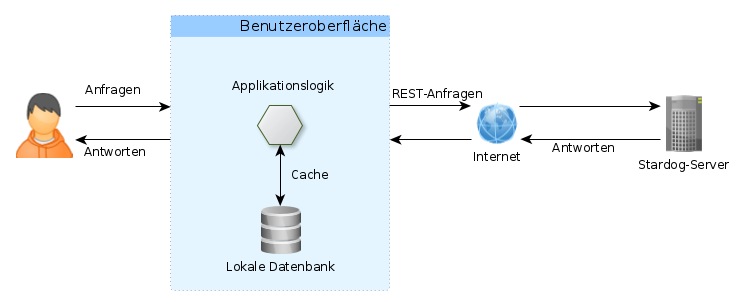
\includegraphics{bilder/architektur_gui.png}}}
    \caption{Architektur der Benutzeroberfläche\label{fig:architektur:gui}\protect\footnotemark}
\end{figure}
\footnotetext{Eigene Darstellung mittels yEd.}

Die obenstehende Abbildung~\ref{fig:architektur:gui} zeigt die Architektur der Benutzeroberfläche, bestehend aus einem Frontend und einem Backend. Bei dem Frontend ist die Applikation selbst gemeint, bei dem Backend handelt es sich um Stardog.

Die Applikation besteht aus \textit{Models}, \textit{Views} und \textit{Routen}.

Die \textit{Models} sind \textit{Reisen}, \textit{Dateneigenschaften} sowie \textit{Objektrelationen}. Die \textit{Models} entsprechen \textit{Individuen}, \textit{DataProperties} und \textit{ObjectProperties} der Ontologie.

Die \textit{Routen} definieren, wie deren Name sagt, den Ablauf der Applikation. Der Einstiegspunkt der Applikation ist die \textit{Welcome}-Rotue. Von dieser aus werden die \textit{Routen} \textit{Step1}, \textit{Step2} und \textit{Step3} nacheinander in Form eines Schritt-für-Schritt-Assistenten durchlaufen. In Schritt 1 wird die Art der Ausflüge gewählt. Da in diesem Schritt nur bestimmte Individuen der Ontologie angezeigt werden sollen, wurden diese in der Ontologie mit der \textit{Dateneigenschaft} ``reise'' gekennzeichnet. So können explizit diese Individuen abgefragt werden. In Schritt 2 werden die \textit{Dateneigenschaften} sowie die \textit{Objektrelationen} pro zuvor gewählter Art der Ausflüge gewählt. Schritt 3 gibt alle Instanzen zurück, welche den gewählten Kriterien entsprechen.

Die \textit{Views} kombinieren die Gestaltung (das Layout) der Seite mit der Ansicht der aktuellen Route.

Die Applikation verfügt über keine dedizierte Datenbank zur Speicherung von Entitäten, zum Beispiel im üblichen Sinne eines Backends. Dies war ein bewusster Entscheid, da in diesem Falle die Ontologie das Backend bzw.\ die Datenbank darstellt und die Ontologie daher hätte verändert werden können. Alternativ dazu hätte die Ontologie nach dem Abfüllen in Objekte gespeichert werden können. Dies bedeutet jedoch viel Aufwand zur Synchronisation bei Änderungen der Ontologie und wurde daher verworfen.

Da die Applikation mit Ember.js umgesetzt wurde und es sich dabei um ein clientseitiges Framework handelt, wird die Applikation bei jedem Aufruf an den Client (Benutzer) übertragen und dort (lokal) ausgeführt. Dies hat zur Folge, dass bei jedem Aufruf der Applikation ein Zugriff auf die Ontologie erfolgt. Die zurückgegebene Ontologie wird lokal zwischengespeichert. Der Zugriff auf die Ontolgie erfolgt per REST-Schnittstelle über das HTTPS-Protokoll via Internet.

Bedingt durch die genannten Gegebenheiten erfolgt der Datenaustausch via Internet. Damit der Benutzer nicht auf den Datenaustausch warten muss und die Applikation blockiert wird, findet der Datenaustausch asynchron statt. Während die Anfrage im Hintergrund läuft, kann die Applikation weiterhin benützt werden. Dabei werden die \textit{Models} an die \textit{Views} gebunden. 

Erhält die Applikation die Daten eines Models, wird automatisch deren \textit{View} dargestellt bzw. aktualisiert.
